\documentclass{standalone}

\usepackage{tikz}
\usetikzlibrary{positioning}


\begin{document}

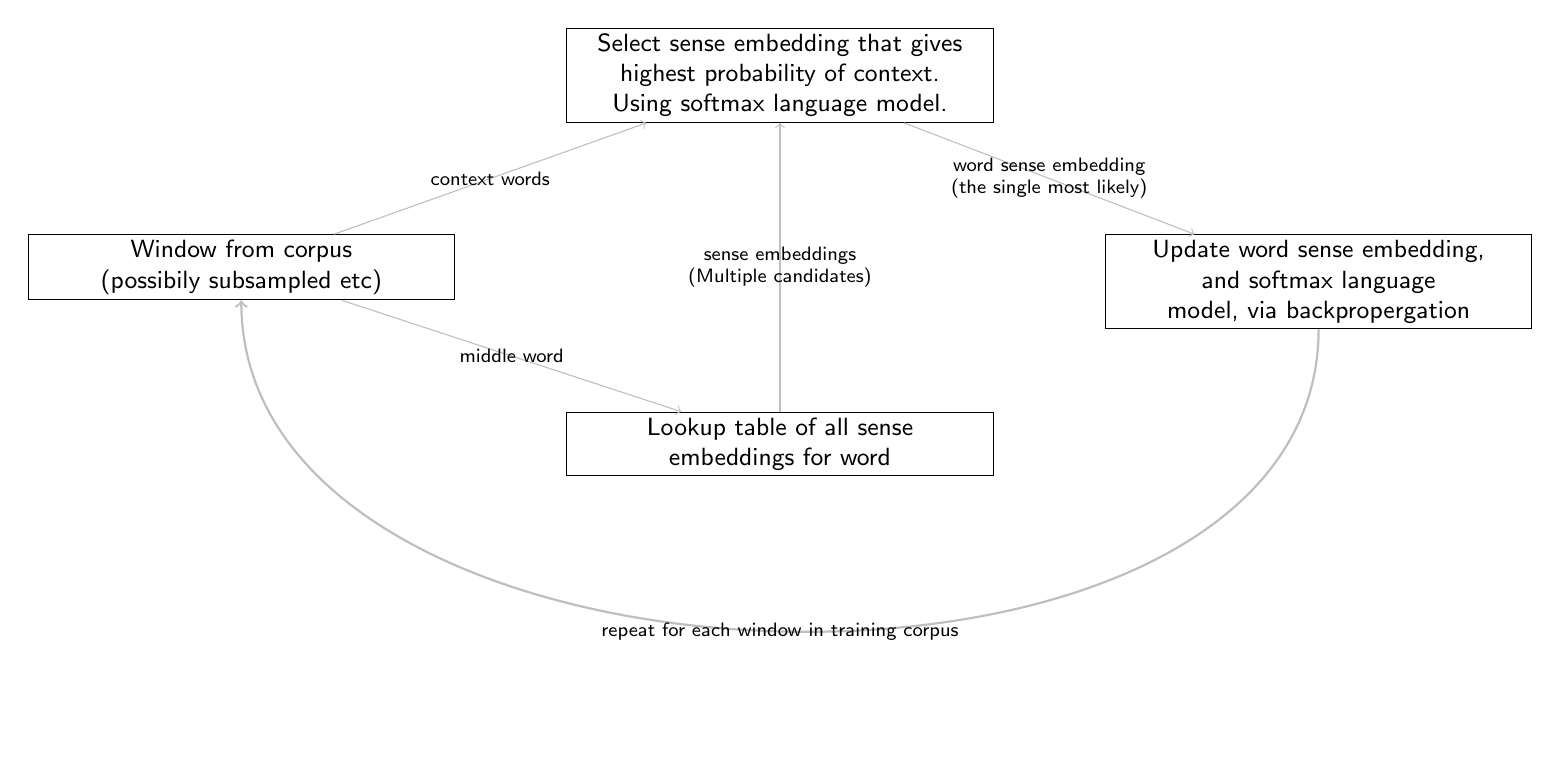
\begin{tikzpicture}[
 	->/.style={lightgray, arrows=->},
	every node/.style={ black,text width=15em,
    					align=center,
                        font=\scriptsize\sffamily,
                        inner sep=1pt
                        },
	proc/.style= {draw,
    			  font=\small\sffamily,
                  inner sep = 2pt
    }
]
	\hyphenpenalty=10000
	\node (window) [proc] {Window from corpus (possibily subsampled etc)};
	\node (lookup) [proc, below right= 2 of window] {Lookup table of all sense embeddings for word};
	\node (WSD) [proc, above right= 2 of window] {Select sense embedding that gives highest probability of context. Using softmax language model.};
	\node (train) [proc, below right= 2 of WSD] {Update word sense embedding, and softmax language model, via backpropergation};
    \draw[->] (window) -> node {context words} (WSD);
	\draw[->] (WSD) -- node{word sense embedding \\ (the single most likely)} (train);
    \draw[->] (window) to node{middle word} (lookup);
    \draw[->] (lookup) -- node {sense embeddings \\ (Multiple candidates)} (WSD);
    \draw[->, thick] (train) to [out=270,in=-90]  node{repeat for each window in training corpus}  (window);

\end{tikzpicture}

\end{document}